\documentclass[border=10pt]{standalone}
\usepackage{xcolor}
\usepackage{pgfplots}
\usepackage{tikz}
\begin{document}
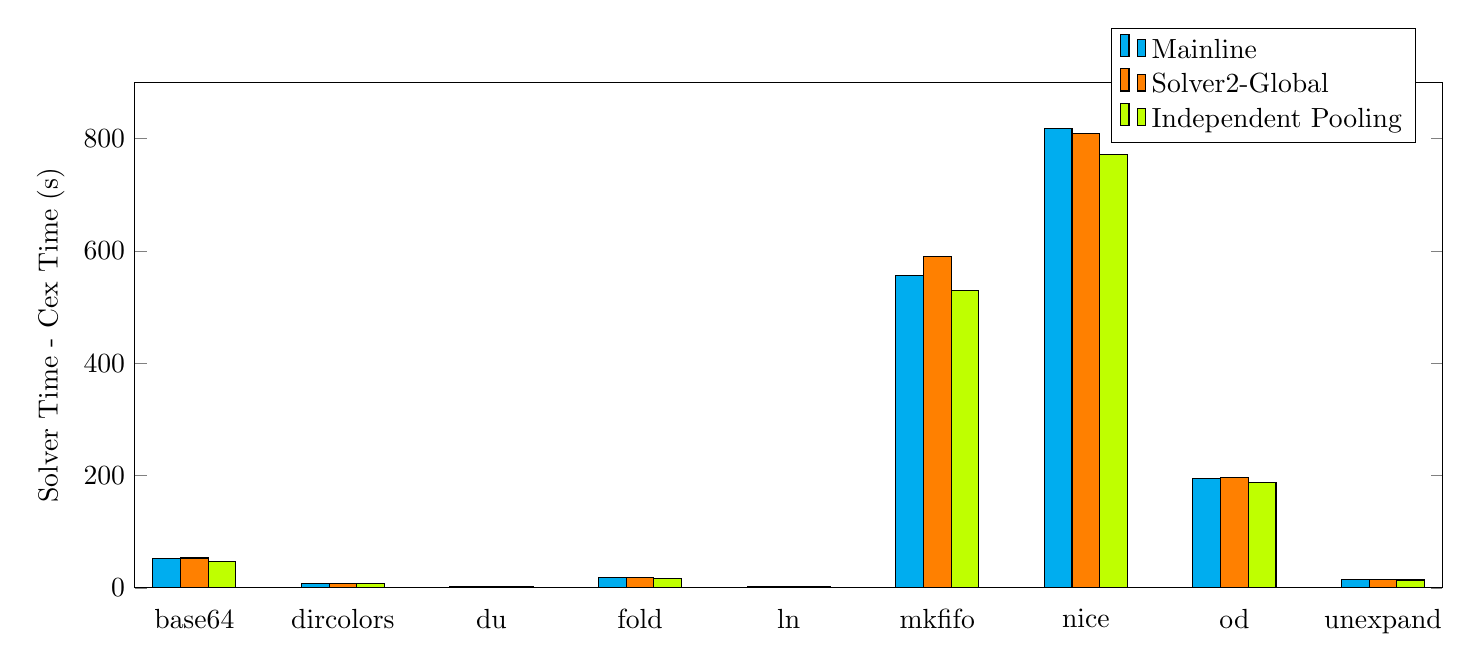
\begin{tikzpicture}
    \begin{axis}[
        width  = 1.5 * \textwidth,
        height = 8cm,
        major x tick style = transparent,
        % tickwidth=10,
        ybar=0,
        bar width=10pt,
        % ymajorgrids = true,
        ylabel = {Solver Time - Cex Time (s)},
        symbolic x coords={base64,dircolors,du,fold,ln,mkfifo,nice,od,unexpand},
        xtick = data,
        scaled y ticks = false,
        enlarge x limits=0.05,
        ymin=0,
        legend cell align=left,
        legend style={
                at={(0.98,0.88)},
                anchor=south east,
                % column sep=1ex
        }
    ]
        \addplot[style={cyan,fill=cyan,mark=none}, draw=black]
	coordinates {(base64,52.61000000000013) (dircolors,7.599999999999454) (du,1.650000000000091) (fold,17.769999999999527) (ln,1.75) (mkfifo,556.6800000000001) (nice,817.87) (od,195.27999999999975) (unexpand,15.099999999999454)};
\addplot[style={orange,fill=orange,mark=none}, draw=black]
	coordinates {(base64,53.25) (dircolors,8.090000000000146) (du,1.6700000000000728) (fold,17.889999999999418) (ln,1.6999999999999886) (mkfifo,589.8399999999999) (nice,809.48) (od,197.15999999999985) (unexpand,15.05999999999949)};
\addplot[style={lime,fill=lime,mark=none}, draw=black]
	coordinates {(base64,47.75) (dircolors,7.579999999999927) (du,1.699999999999818) (fold,16.289999999999964) (ln,1.6899999999999977) (mkfifo,528.71) (nice,771.72) (od,188.08000000000015) (unexpand,14.159999999999854)};

        \legend{Mainline,Solver2-Global,Independent Pooling}
    \end{axis}
\end{tikzpicture}
\end{document}
